%%%%%%%%%%%%%%%%%%%%%%%%%%%%%%%%%%%%%%%%%%%%%%%%%%%%%%%%%%%%%%%%%%%%%%%%%%%%%%%%
%% 
%% このファイル:高知高専専攻科 特別研究中間発表フォーマット 使用例
%% nitkc-senkoka-chukan-sample.tex
%% 
%% 
%% 下記の関連ファイルをこのファイルと同じフォルダに置いてコンパイルしてください
%% 
%% 関連ファイル1:高知高専専攻科 特別研究中間発表フォーマット
%% nitkc-senkoka-chukan.sty
%% 
%% 関連ファイル2:nitkc-senkoka-chukan.sty必須パッケージ群
%% nitkc-senkoka-chukan-preamble.tex
%% 
%% 
%% 下記の関連ファイルを適切な位置に置いてコンパイルしてください
%% 詳細は「latexmk」で検索してください
%% 
%% 関連ファイル3:コンパイル時の設定ファイル
%% .latexmkrc
%% 
%% .latexmkrcの中身は下記の通りです
%% 環境によっては中身を書き換える必要があるかもしれません
%% $latex = 'platex';
%% $bibtex = 'pbibtex';
%% $dvipdf = 'dvipdfmx %O -o %D %S';
%% $makeindex = 'mendex %O -o %D %S';
%% 
%% Overleafを使う場合はファイル名をlatexmkrc(ピリオドなし)として
%% 最上位階層に置いてください(フォルダの中に入れないでください)
%% 
%% 
%% 対応コンパイラ:pLaTeX
%% 文字コード:UTF-8
%% 
%% 諸注意
%% ・本文中で使用するフォントスタイルは既に定義されています
%%  特殊な事情がない限りは,これらのスタイルを使用してください
%%  本文:\TextFont
%% ・その他フォーマットに関する詳細な指定は本文に記述されています
%% 
%%%%%%%%%%%%%%%%%%%%%%%%%%%%%%%%%%%%%%%%%%%%%%%%%%%%%%%%%%%%%%%%%%%%%%%%%%%%%%%%


% 必須な読み込み
\documentclass{jsarticle}
\usepackage{nitkc-senkoka-chukan}
%%%%%%%%%%%%%%%%%%%%%%%%%%%%%%%%%%%%%%%%%%%%%%%%%%%%%%%%%%%%%%%%%%%%%%%%%%%%%%%%
%% 
%% このファイル:nitkc-senkoka-chukan.sty必須パッケージ群
%% nitkc-senkoka-chukan-preamble.tex
%% 
%% 
%% このファイルは下記の関連ファイルと併用することを想定し製作されています.
%% 
%% 関連ファイル1:高知高専専攻科 特別研究中間発表フォーマット
%% nitkc-senkoka-chukan.sty
%% 
%% 
%% 詳しくは下記の関連ファイルを参照してください.
%% 
%% 関連ファイル2:高知高専専攻科 特別研究中間発表フォーマット 使用例
%% nitkc-senkoka-chukan-sample.tex
%% 
%%%%%%%%%%%%%%%%%%%%%%%%%%%%%%%%%%%%%%%%%%%%%%%%%%%%%%%%%%%%%%%%%%%%%%%%%%%%%%%%


% 日本語フォント設定
\usepackage[deluxe, jis2004]{otf}
\usepackage[relfont, usecmapforalphabet]{pxchfon}
\usepackage{graphicx}
\setmediumminchofont{HaranoAjiMincho-Medium.otf} % \mcfamily\mdseries
\setboldminchofont{HaranoAjiMincho-Bold.otf} % \mcfamily\bfseries
\setmediumgothicfont{HaranoAjiGothic-Medium.otf} % \gtfamily\mdseries
\setboldgothicfont{HaranoAjiGothic-Bold.otf} % \gtfamily\bfseries



% 任意な読み込み
% ここに\usepackageを記述
% 下記のパッケージは既にnitkc-senkoka-chukan-preamble.texで読み込み済み
% ・otf, pxchfon, graphicx
\usepackage{amsmath, amssymb}


% タイトル
\title{高知高専専攻科 特別研究中間発表フォーマット\\使用例}

% 著者:文字間はすべて全角スペース
\author{山 田 太 郎}

% 所属専攻
\department{機械・電気工学専攻}

% 所属研究室
\affiliate{山田研究室}

% キーワード:区切りは全角コンマ
\keywords{キーワード1,キーワード2,Keyword3}


% 文書の開始
\begin{document}

% タイトル,著者,所属専攻,所属研究室,キーワードを出力
\maketitle


% ここから本文
\section{緒  言}
このフォーマットは,特別研究中間発表会要旨の独自製作{\LaTeX}フォーマットです.このフォーマットの開発はGitHub(https://github.com/ebifly5011/nitkc-tex)で行われています.是非アイデアやご意見をお寄せください.

{\LaTeX}の基本操作や環境設定,書きかたなどはWeb情報がありますのでそちらをご覧ください.

\section{利用方法}
引用例\citations{\cite{zasshisample}〜\cite{tankoubon}}.

図の例をFig.\ref{fig:sample}に示す.

\begin{figure}[htbp]
\centering
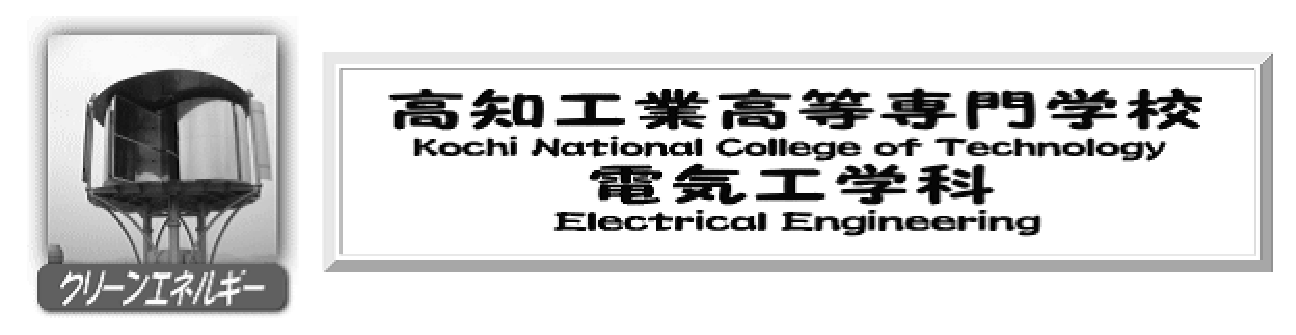
\includegraphics[width=\columnwidth]{KNCT-EE.eps}
\caption{figure sample}
\label{fig:sample}
\end{figure}

表の例をTable \ref{tab:sample}に示す.

\begin{table}[htbp]
\centering
\caption{table sample}
\label{tab:sample}
\begin{tabular}{c|c}
\hline \hline
col1 & col2 \\
\hline
dat1 & dat2 \\
dat3 & dat4 \\
\hline \hline
\end{tabular}
\end{table}

図表中の語句・説明文は英語(9pt,Times New Roman)にしてください.
変数名はイタリックにしてください.
\section{結  言}


\section*{謝  辞}
ありがとうございました.

\begin{thebibliography}{99}
\bibitem{zasshisample}
越智義明,中島保雄,金属材料の長寿命疲労研究の動向と今後の課題,日本材料学会誌,{\bfseries 64},11(1997),pp.43-48.

\bibitem{tankoubonsample}
村上敬宜,金属疲労,養賢堂,(1993),pp.1-9,pp.73-152.

\bibitem{zasshi}
著者名,タイトル,雑誌名,{\bfseries 巻},号(発行西暦年), 開始-最終ページ.

\bibitem{tankoubon}
著者名,書名,発行所,(発行西暦年),pp.開始-最終ページ.
\end{thebibliography}

\end{document}
